% ============================================================================
%  E-BOOK DIDÁTICO — EMPREENDEDORISMO E ANÁLISE MERCADOLÓGICA
%  Material de apoio à 4ª Entrega · Imersão ODS
%  ETE Cícero Dias — Curso Técnico em Desenvolvimento de Sistemas
%
%  Estilo: padrão de template da disciplina (REVESTU) + didática MJV.
%  Compilação: pdflatex (2x) — compatível com Overleaf e Google Colab.
% ============================================================================
\documentclass[11pt, a4paper]{article}

% ---------- Codificação e idioma ----------
\usepackage[utf8]{inputenc}
\usepackage[T1]{fontenc}


% ---------- Geometria: margens generosas, texto centralizado (estilo MJV) ----------
\usepackage[
  top=2.8cm, bottom=2.8cm,
  left=3.6cm, right=3.6cm,   % colunas laterais = respiro visual
  headheight=14pt
]{geometry}

% ---------- Tipografia — Helvetica/Nimbus (Vista Sans do MJV) ----------
\usepackage[scaled=0.96]{helvet}
\renewcommand{\familydefault}{\sfdefault}
\usepackage{microtype}
\usepackage{setspace}
\setstretch{1.18}   % entrelinha levemente aberta, mais legível

% ---------- Recursos gráficos e tabelas ----------
\usepackage{graphicx}
\usepackage{array}
\usepackage{booktabs}
\usepackage{enumitem}
\usepackage{float}
\usepackage{caption}
\usepackage{framed}
\usepackage{lettrine}
\usepackage{ragged2e}
\usepackage{tabularx}
\usepackage{multirow}

% ---------- Cores ----------
\usepackage{xcolor}
\usepackage{colortbl}

% ---------- Layout, capa e títulos ----------
\usepackage{tikz}
\usepackage{eso-pic}
\usepackage{titlesec}
\usepackage{fancyhdr}
\usepackage{xurl}
\usepackage[hidelinks]{hyperref}

% ============================================================================
%  PALETA  (vinho/creme/sálvia da capa + vermelho MJV para abertura de seção)
% ============================================================================
\definecolor{wineDeep}{HTML}{5C1519}
\definecolor{wine}{HTML}{7A1F1E}
\definecolor{redAccent}{HTML}{BC3B2C}   % vermelho rótulos
\definecolor{redMJV}{HTML}{E63229}      % vermelho vivo blocos de seção (igual MJV)
\definecolor{sage}{HTML}{828C52}
\definecolor{sageSoft}{HTML}{A6AE78}
\definecolor{cream}{HTML}{F1EBDD}
\definecolor{creamMid}{HTML}{E5DECC}
\definecolor{ink}{HTML}{1A1A1A}
\definecolor{slate}{HTML}{6E5F5F}
\definecolor{lightgray}{HTML}{F4F4F4}

\hypersetup{
  colorlinks=true, linkcolor=wineDeep, urlcolor=wine, citecolor=wine,
  breaklinks=true,
  pdftitle={Empreendedorismo e Análise Mercadológica — E-book da 4ª Entrega},
  pdfauthor={Samara Silvia Sabino}
}

% ============================================================================
%  DADOS DO MATERIAL
% ============================================================================
\newcommand{\matTitulo}{Empreendedorismo e Análise Mercadológica}
\newcommand{\matSubtitulo}{Material de apoio teórico à 4ª entrega do Projeto Integrador}
\newcommand{\matEtapa}{Imersão ODS \textbullet\ Entrega 4}
\newcommand{\matCurso}{Técnico em Desenvolvimento de Sistemas}
\newcommand{\matInstituicao}{ETE Cícero Dias}
\newcommand{\matAutora}{Samara Silvia Sabino}
\newcommand{\matData}{Recife, junho de 2026}

% ============================================================================
%  ABERTURA DE SEÇÃO — estilo MJV
%  Título grande em wineDeep, seguido de linha fina redAccent
%  (a página de abertura com bloco colorido é feita via \aberturaSecao)
% ============================================================================

% \novaSecao{título}{subtítulo-breve}
% Gera uma página de abertura com bloco de cor, título branco grande e lead
\newcommand{\novaSecao}[2]{%
  \clearpage
  \thispagestyle{empty}%
  \begin{tikzpicture}[remember picture, overlay]
    % bloco colorido cobre ~55% da altura da página
    \fill[redMJV]
      (current page.north west)
      rectangle
      ([yshift=-0.54\paperheight]current page.north east);
    % título branco
    \node[anchor=north west,
          text=white,
          font=\sffamily\bfseries\fontsize{44}{50}\selectfont,
          text width=0.62\paperwidth,
          align=left,
          inner sep=0]
      at ([xshift=3.6cm, yshift=-2.8cm]current page.north west)
      {#1};
    % subtítulo / lead
    \node[anchor=north west,
          text=white,
          font=\sffamily\fontsize{14}{19}\selectfont,
          text width=0.62\paperwidth,
          align=left,
          inner sep=0]
      at ([xshift=3.6cm, yshift=-0.42\paperheight]current page.north west)
      {#2};
  \end{tikzpicture}%
  \vspace*{0.57\paperheight}%
  % NÃO faz segundo clearpage — conteúdo começa logo abaixo na mesma página
}

% \section reformatado: título grande no topo da página de conteúdo
\titleformat{\section}[block]
  {\normalfont\sffamily\bfseries\fontsize{28}{32}\selectfont\color{ink}}
  {}{0pt}{}[\vspace{4pt}{\color{redAccent}\rule{\linewidth}{1.4pt}}\vspace{12pt}]
\titlespacing*{\section}{0pt}{0pt}{18pt}

\titleformat{\subsection}
  {\normalfont\sffamily\bfseries\large\color{wineDeep}}
  {}{0pt}{}
\titlespacing*{\subsection}{0pt}{16pt}{4pt}

% ============================================================================
%  RÓTULO DIDÁTICO — estilo MJV duas colunas, SEM minipage
%  A barra vermelha e o label ficam na margem esquerda via \marginnote-like trick
%  Implementação: recuo de parágrafo + label inline à esquerda
%
%  Uso: \rotulo{O que é}
%  \fimRotulo — NÃO é mais necessário (mantido como \relax para compatibilidade)
% ============================================================================
\newcommand{\rotulo}[1]{%
  \par\vspace{16pt}%
  \noindent
  \begin{tikzpicture}[remember picture, overlay]
    \draw[color=redAccent, line width=1.2pt]
      ([xshift=-1.5cm, yshift=0.2ex]0,0) -- ([xshift=-1.5cm, yshift=-1.6em]0,0);
    \node[anchor=north east, text=redAccent,
          font=\sffamily\bfseries\fontsize{7}{8}\selectfont,
          align=right, text width=1.25cm]
      at ([xshift=-1.65cm, yshift=0.15ex]0,0)
      {\MakeUppercase{#1}};
  \end{tikzpicture}%
  \ignorespaces
}

% fimRotulo — mantido como no-op para não quebrar o documento
\newcommand{\fimRotulo}{\par\vspace{2pt}}

% ============================================================================
%  CAIXA DE DESTAQUE — fundo sólido redMJV, texto branco (estilo MJV real)
% ============================================================================
\newenvironment{caixaDestaque}{%
  \par\vspace{10pt}%
  \noindent\colorbox{redMJV}{%
    \begin{minipage}{\dimexpr\linewidth-2\fboxsep\relax}%
      \setlength{\parskip}{5pt}%
      \vspace{8pt}%
      \color{white}\sffamily\small%
}{%
      \vspace{8pt}%
    \end{minipage}%
  }\par\vspace{10pt}%
}

% ---------- Citação com barra lateral (para citações de autores) ----------
\newenvironment{citacaoBox}{%
  \par\vspace{6pt}%
  \def\FrameCommand{{\color{redAccent}\vrule width 3pt}\hspace{14pt}}%
  \MakeFramed{\advance\hsize-\width\FrameRestore}%
  \small\itshape\color{ink!80}%
}{%
  \par\endMakeFramed\vspace{6pt}%
}
\newcommand{\citacaoDestaque}[2]{%
  \begin{citacaoBox}#1\par\vspace{4pt}%
    {\normalfont\footnotesize\color{slate}\hfill\textsc{\textemdash{}\,#2}}%
  \end{citacaoBox}%
}

% ============================================================================
%  CABEÇALHO E RODAPÉ — estilo MJV: mínimo, rodapé com seção + número
% ============================================================================
\fancypagestyle{corpo}{%
  \fancyhf{}
  \renewcommand{\headrulewidth}{0pt}   % sem linha de header — mais limpo
  \fancyfoot[L]{\footnotesize\sffamily\textcolor{slate!70}{\leftmark}}
  \fancyfoot[R]{\footnotesize\sffamily\textcolor{ink}{\textbf{\thepage}}}
}
\renewcommand{\sectionmark}[1]{\markboth{#1}{}}

% ---------- Macro do Lean Canvas (caixa) — mantida, usada no diagrama ----------
\newcommand{\cvbox}[7]{%
  \draw[fill=cream, draw=sageSoft, line width=0.8pt] (#1,#2) rectangle (#1+#3,#2+#4);
  \node[anchor=north west, text width=\dimexpr #3cm-12pt\relax, align=left, inner sep=0pt]
       at (#1+0.2,#2+#4-0.2)
       {{\sffamily\bfseries\scriptsize\color{sage}#5\,\textbullet\,}{\sffamily\bfseries\footnotesize\color{wineDeep}#6}\\[3pt]%
        {\color{ink!75}\scriptsize #7}};%
}

% ---------- Referências ----------
\newcommand{\refnum}[1]{\textcolor{wineDeep}{\sffamily\bfseries[#1]}\ }

\setlength{\parskip}{7pt}
\setlength{\parindent}{0pt}

% Nomes de legenda em PT
\renewcommand{\figurename}{Figura}
\renewcommand{\tablename}{Tabela}

% ============================================================================
\begin{document}

% ----------------------------------------------------------------------------
%  CAPA — imagem em página inteira (capa-mercado.png)
% ----------------------------------------------------------------------------
\begin{titlepage}
\thispagestyle{empty}
\begin{tikzpicture}[remember picture, overlay]
  \node at (current page.center)
    {
\includegraphics[width=\paperwidth, height=\paperheight]{imgs/capa-mercado.png}};
\end{tikzpicture}
\end{titlepage}

% ----------------------------------------------------------------------------
%  FOLHA DE ROSTO
% ----------------------------------------------------------------------------
\thispagestyle{empty}
\vspace*{2.4cm}
\begin{center}
  {\sffamily\footnotesize\color{slate} \MakeUppercase{\matEtapa}}\\[0.45cm]
  {\color{sageSoft}\rule{2.4cm}{1.2pt}}\\[1.0cm]

  {\sffamily\bfseries\color{ink}\fontsize{40}{44}\selectfont \matTitulo}\\[0.7cm]
  {\itshape\large\color{wineDeep} \matSubtitulo}\\[2.6cm]

  {\sffamily\color{slate}\large Material didático}\\[0.4cm]
  {\sffamily\color{ink}\large \matCurso}
\end{center}

\vfill

\begin{center}
  {\color{sageSoft}\rule{0.42\textwidth}{0.5pt}}\\[0.7cm]
  {\sffamily\footnotesize\color{slate}
    \matInstituicao\\[3pt]
    Profa.\ \matAutora\\[3pt]
    \matData}
\end{center}
\vspace{1.2cm}
\clearpage

% ----------------------------------------------------------------------------
%  SOBRE A AUTORA  (quem produziu o material + foto)
% ----------------------------------------------------------------------------
\thispagestyle{empty}
\vspace*{1.2cm}

{\centering\sffamily\footnotesize\color{sage} SOBRE A AUTORA\par}
\vspace{0.28cm}
{\centering\sffamily\bfseries\fontsize{34}{34}\selectfont\color{ink} Quem produziu este material\par}
\vspace{0.28cm}
{\centering{\color{sageSoft}\rule{2.6cm}{1.2pt}}\par}
\vspace{0.9cm}

\begin{center}
  \begin{tikzpicture}
    \node[circle, draw=sageSoft, line width=1.5pt, minimum size=3.2cm, inner sep=0,
          path picture={\node at (path picture bounding box.center)
            {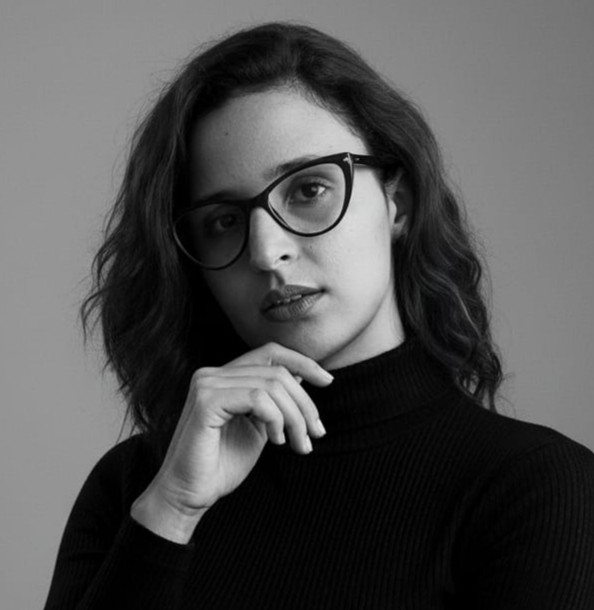
\includegraphics[width=3.5cm]{imgs/avatar-samara.jpg}};}] {};
  \end{tikzpicture}\\[0.5cm]
  {\sffamily\bfseries\large\color{wineDeep} \matAutora}\\[3pt]
  {\sffamily\footnotesize\color{slate} Desenvolvedora Frontend \textperiodcentered\ UX/UI \textperiodcentered\ Mestranda em Ciência da Computação (CIn/UFPE)}
\end{center}

\vspace{0.9cm}
\begin{center}
\begin{minipage}{0.82\textwidth}
\setlength{\parskip}{6pt}\color{ink}\justifying
Este material didático foi elaborado por \matAutora, professora do Curso
\matCurso\ da \matInstituicao. Reúne os fundamentos teóricos que sustentam a
4ª entrega do projeto integrador \textemdash{} a etapa de \textbf{análise
mercadológica} \textemdash{}, na qual cada solução desenvolvida ao longo da
Imersão ODS passa a ser examinada sob a perspectiva de negócio e de mercado.

A proposta deste documento é \textbf{substituir a aula expositiva por um texto
de estudo}: em vez de tópicos de slide, apresentam-se aqui os conceitos
desenvolvidos com a profundidade de um capítulo de livro, recuperando a origem
histórica de cada ferramenta e explicando por que ela é produzida no projeto.
A leitura deve preceder a execução dos artefatos da entrega.
\end{minipage}
\end{center}
\vspace{0.8cm}
\clearpage

% ----------------------------------------------------------------------------
%  SUMÁRIO
% ----------------------------------------------------------------------------
\thispagestyle{empty}
\renewcommand{\contentsname}{\normalfont\sffamily\bfseries\color{wineDeep}\Huge Sumário}
{\hypersetup{linkcolor=ink}\tableofcontents}
\clearpage

% ----------------------------------------------------------------------------
%  APRESENTAÇÃO
% ----------------------------------------------------------------------------
\pagestyle{corpo}

\begin{center}
  {\sffamily\footnotesize\color{sage} \MakeUppercase{Apresentação}}\\[6pt]
  {\sffamily\bfseries\color{wineDeep}\fontsize{28}{32}\selectfont Por que analisar o mercado?}\\[8pt]
  {\color{sageSoft}\rule{2.4cm}{1pt}}
\end{center}
\vspace{0.7cm}

{\color{ink}\justifying
\lettrine[lines=3, lhang=0.08, findent=3pt, nindent=8pt]{\color{wineDeep}\sffamily A}{o}
longo da Imersão ODS, cada grupo percorreu um caminho de descoberta genuína:
mergulhou em um problema real ligado a um Objetivo de Desenvolvimento
Sustentável, investigou as pessoas afetadas, prototipou e reformulou. Até
aqui, o olhar esteve voltado para \textit{dentro} da solução. A 4ª entrega
inaugura uma virada: a ideia construída passa a ser confrontada com o
\textbf{mundo exterior}, ou seja, com o mercado em que ela pretenderia existir.

Essa virada não é burocrática. Ela é necessária \textemdash{} e muitas vezes
incômoda. Uma solução pode ser tecnicamente elegante e ainda assim não encontrar
lugar no mundo: porque já existe alguém que resolve o mesmo problema com mais
recursos, porque o público-alvo não percebe valor suficiente para mudar de
comportamento, ou porque o modelo de sustentação não se sustenta. A análise
mercadológica é o instrumento que torna esses riscos visíveis antes que tempo e
esforço sejam investidos em uma direção equivocada.

Você vai estudar, neste material, quatro ferramentas que trabalham juntas:
o \textbf{benchmarking}, que mapeia quem já atua no espaço;
a \textbf{pesquisa desk}, que documenta o estado real do mercado a partir de
fontes secundárias;
o \textbf{Lean Canvas}, que sintetiza o modelo de negócio da solução em uma
única página;
e a análise do \textbf{diferencial competitivo}, que articula o que torna a
proposta preferível às alternativas.

Cada seção apresenta o conceito, sua origem histórica, tipos relevantes e pelo
menos um exemplo concreto. A leitura deve preceder a execução \textemdash{} não
porque as ferramentas sejam difíceis, mas porque entender \textit{por que} se
usa uma ferramenta é o que transforma preenchimento mecânico em análise real.
\par}

% ============================================================================
\novaSecao{O que é empreendedorismo}{Empreender é identificar uma oportunidade onde outros veem apenas o estado das coisas — e agir.}
% ============================================================================

O termo \textbf{empreendedorismo} é frequentemente reduzido, no senso comum, à
ideia de ``abrir um negócio''. Essa leitura é estreita demais. Empreender, em
sentido pleno, é o ato de identificar uma oportunidade onde outros enxergam
apenas o estado das coisas \textemdash{} e mobilizar recursos para transformar
essa oportunidade em valor concreto: um produto, um serviço, uma política, uma
solução.

O empreendedor não é necessariamente quem inventa algo do zero. É quem
\textit{realiza} a inovação: percebe que algo pode ser feito de forma diferente,
reúne os meios para fazê-lo e age. Essa distinção é importante porque coloca o
empreendedorismo ao alcance de qualquer contexto \textemdash{} inclusive o de
um projeto escolar.

\rotulo{De onde vem o conceito}

A formulação mais influente do empreendedor como agente de transformação vem do
economista austríaco \textbf{Joseph Schumpeter} (1883--1950). Para ele, o
empreendedor é o motor das chamadas ``novas combinações'': introduz produtos,
métodos produtivos, mercados ou formas organizacionais inéditos e, ao fazê-lo,
desloca o equilíbrio econômico vigente. Schumpeter chamou esse processo de
\textbf{destruição criativa}: o novo não convive pacificamente com o velho
\textemdash{} ele o substitui.

\citacaoDestaque{O empreendedor não é necessariamente o inventor, mas aquele que
realiza a inovação: transforma uma possibilidade em prática econômica
concreta.}{síntese do pensamento de Schumpeter (1934)}

Décadas depois, \textbf{Peter Drucker} (1909--2005) tornou o conceito
ainda mais prático. Para Drucker, a inovação é uma \textit{disciplina} que
pode ser aprendida e praticada sistematicamente \textemdash{} não um lampejo
de genialidade. Empreender, nessa leitura, é observar mudanças no ambiente,
identificar a lacuna que elas abrem e agir sobre ela com método.

Mais recentemente, \textbf{Eric Ries} e \textbf{Steve Blank} desenvolveram
metodologias voltadas a projetos em estágio inicial: a \textit{Lean Startup}
e o \textit{Customer Development}. A premissa central de ambas é que, no início
de qualquer empreendimento, tudo que existe são hipóteses \textemdash{} e o
papel do empreendedor é testá-las o mais rápido e barato possível, antes de
investir pesado em uma direção que pode estar errada.

\fimRotulo
\rotulo{Empreendedorismo no mundo real}

Vejamos dois exemplos que ilustram o conceito além da teoria:

\textbf{Netflix (1997).} Reed Hastings e Marc Randolph observaram uma dor
real: as multas abusivas das locadoras de vídeo. A solução inicial não foi o
streaming, mas o aluguel de DVDs por correio, sem multa por atraso. O mercado
já existia \textemdash{} a Blockbuster dominava. O que mudou foi o modelo de
entrega e a política de cobrança. Anos depois, ao perceber a chegada da banda
larga, a Netflix reinventou seu próprio negócio antes de ser reinventada por
outro. Destruição criativa aplicada a si mesma.

\textbf{iFood (2011).} O problema identificado era simples: pedir comida por
telefone era lento, impreciso e sem rastreabilidade. A solução \textemdash{}
um marketplace digital de delivery \textemdash{} não inventou restaurantes
nem comida. Reorganizou quem acessa quem, e como. O diferencial não era
tecnológico puro: era a \textit{fricção eliminada} no processo de pedido.

Em ambos os casos, o ponto de partida foi uma \textbf{dor real de um público
real} \textemdash{} não uma tecnologia em busca de uso. Essa inversão de
raciocínio é central ao empreendedorismo contemporâneo.

\fimRotulo
\rotulo{Por que isso importa no projeto}

O projeto integrador é, em escala, um exercício de empreendedorismo. Os grupos
não recebem um problema resolvido: identificam uma oportunidade dentro de um ODS
e constroem uma resposta. A 4ª entrega não abandona esse espírito \textemdash{}
ela o aprofunda. Agora a pergunta não é apenas ``o que fazemos?'', mas ``por que
alguém adotaria o que fazemos?''. É a mentalidade empreendedora que dá sentido
a essa pergunta \textemdash{} e é a análise mercadológica que oferece os
instrumentos para respondê-la.

\fimRotulo
% ============================================================================
\novaSecao{Por que a análise mercadológica}{Antes de construir, é preciso entender o mercado em que a solução pretende existir.}
% ============================================================================

\textbf{Análise mercadológica} é o estudo sistemático do ambiente de mercado
em que uma solução pretende se inserir. Ela investiga quem já atua nesse
espaço, o que o público efetivamente demanda, quais lacunas permanecem abertas
e o que tornaria uma nova proposta competitiva. Em essência, é a validação de
uma ideia pela \textit{lente do mercado e do negócio}: não ``o que queremos
construir'', mas ``há lugar para o que queremos construir?''.

\rotulo{De onde vem o conceito}

A análise sistemática de mercado consolidou-se com o desenvolvimento do
\textbf{marketing} como campo de estudo. \textbf{Philip Kotler} estruturou a
compreensão de mercados, segmentos e necessidades do consumidor de forma
rigorosa, mostrando que uma organização que não conhece seu mercado está
navegando sem bússola.

À leitura de mercado soma-se a perspectiva da \textbf{estratégia competitiva},
de \textbf{Michael Porter}: toda organização opera em um ambiente de forças
concorrenciais, e seu desempenho depende da posição que ocupa em relação a
essas forças. Conhecer os concorrentes não é opcional \textemdash{} é o ponto
de partida de qualquer decisão estratégica.

\fimRotulo
\rotulo{As três perguntas da etapa}

A análise mercadológica de um projeto pode ser resumida em três perguntas que
orientam toda a 4ª entrega:

\begin{enumerate}[leftmargin=1.6em, itemsep=4pt, label=\textcolor{sage}{\textbf{\arabic*.}}]
  \item A solução é \textbf{viável}? Existe um público disposto a adotá-la, e
        um caminho para que ela se sustente?
  \item Já existe \textbf{algo semelhante}? Quem mais atua sobre o mesmo
        problema, de forma direta ou indireta?
  \item O que \textbf{diferencia} a solução das alternativas existentes?
        Por que alguém escolheria esta proposta e não outra?
\end{enumerate}

Nenhuma dessas perguntas é de ordem técnica. Todas dizem respeito à inserção
da solução na realidade. Para respondê-las, produzem-se quatro artefatos,
tratados nas seções seguintes: o \textit{benchmarking}, a pesquisa desk, o
Lean Canvas e a análise do diferencial competitivo.

\fimRotulo
\rotulo{Por que isso importa antes de prototipar}

Considere o Orkut. Lançado pelo Google em 2004, chegou a ser a maior rede
social do Brasil \textemdash{} com 28 milhões de usuários nacionais em seu
pico. Encerrou em 2014. O que aconteceu? Em parte, a falta de adaptação ao
comportamento real dos usuários móveis e às demandas de privacidade que o
Facebook soube capturar melhor. Não foi uma falha técnica: foi uma falha de
\textit{leitura de mercado em movimento}.

O exemplo ilustra por que a análise mercadológica não é exercício burocrático:
ela é o que separa uma solução que existe de uma solução que \textit{persiste}.
No projeto de vocês, o esforço é proporcional \textemdash{} mas o raciocínio
é exatamente o mesmo.

\fimRotulo
% ============================================================================
\novaSecao{Benchmarking}{Comparar sistematicamente é a única forma de saber onde está a oportunidade real.}
% ============================================================================
\rotulo{O que é}
\textit{Benchmarking} é o processo de comparar sistematicamente uma solução com
referências do mercado \textemdash{} concorrentes e organizações reconhecidas
\textemdash{} a fim de identificar pontos fortes, pontos fracos e oportunidades
de aperfeiçoamento. O termo deriva de \textit{benchmark}, a marca de referência
usada em topografia como ponto fixo de medição: sabe-se onde se está porque se
sabe onde está o ponto fixo.

Aplicado a projetos de negócio ou de produto digital, o benchmarking responde
à pergunta: \textbf{em relação às alternativas existentes, onde está a
oportunidade?}

\fimRotulo
\rotulo{De onde vem}
A prática foi formalizada pela \textbf{Xerox} no final da década de 1970.
Diante da perda de participação de mercado para concorrentes japoneses,
a empresa passou a comparar seus processos internos com os das líderes de cada
setor \textemdash{} não apenas da indústria de impressão. A sistematização
do método foi publicada por \textbf{Robert Camp} em 1989, estabelecendo o
benchmarking como ferramenta estruturada de gestão.

\fimRotulo
\rotulo{Tipos de benchmarking}
Nem todo benchmarking é igual. Dependendo do objetivo, utiliza-se um tipo
diferente:

\begin{itemize}[leftmargin=1.4em, itemsep=5pt, label=\textcolor{sage}{\textbf{\textbullet}}]
  \item \textbf{Benchmarking competitivo} — comparação direta com concorrentes
    que disputam o mesmo mercado. É o mais imediato: o que o concorrente
    faz, qual o preço, quais as funcionalidades, onde ele falha.
    \textit{Exemplo:} um app de gestão financeira pessoal comparando-se com
    Mobills, GuiaBolso e Organizze.

  \item \textbf{Benchmarking funcional} — comparação de funções específicas
    com empresas de setores distintos que as executam de forma exemplar.
    \textit{Exemplo:} uma startup de saúde estudando o sistema de onboarding
    do Nubank para melhorar o seu próprio fluxo de cadastro, mesmo que o
    Nubank não atue em saúde.

  \item \textbf{Benchmarking de UX / experiência} — análise comparativa da
    experiência do usuário em produtos concorrentes ou de referência. Examina
    fluxos de navegação, padrões de interface, consistência visual, acessibilidade,
    tom de voz, onboarding e pontos de fricção. É o tipo mais relevante para
    projetos de produto digital.
    \textit{Exemplo:} uma equipe desenvolvendo um app de doação de alimentos
    analisa os fluxos de doação do Doe Seu Livro, do Vakinha e do Catarse
    \textemdash{} produtos que não são concorrentes diretos, mas que ensinam
    como facilitar a ação de contribuir.
\end{itemize}

\fimRotulo
\rotulo{Concorrentes diretos e indiretos}
A comparação distingue dois tipos de concorrente. O \textbf{concorrente direto}
oferece essencialmente a mesma solução ao mesmo público. O \textbf{concorrente
indireto} resolve o mesmo problema por um caminho distinto. A omissão dos
concorrentes indiretos é uma das falhas mais frequentes \textemdash{} e é
justamente neles que costuma residir a concorrência mais real. Quando o Spotify
chegou ao Brasil, o concorrente mais perigoso não era outro app de streaming:
era o hábito de ouvir rádio AM/FM.

\fimRotulo
\rotulo{Exemplo real de benchmarking de UX}

O time de design do iFood realizou benchmarking contínuo com Uber Eats e
Rappi, mas também com apps de e-commerce como Magalu e Americanas. O objetivo
era entender como telas de lista e detalhe de produto funcionavam em contextos
de decisão rápida. O resultado informou redesenhos no fluxo de seleção de
restaurante e nos filtros de busca \textemdash{} melhorias que não vinham de
comparação direta com concorrentes, mas de referências de setores adjacentes.

\fimRotulo
\rotulo{Como aplicar}
O benchmarking se materializa em uma \textbf{tabela comparativa}, na qual cada
concorrente é avaliado segundo critérios relevantes ao problema. A
Tabela~\ref{tab:bench} ilustra o formato, com critérios aplicados a um tema de
moda sustentável.

\begin{table}[H]
\centering
\small
\renewcommand{\arraystretch}{1.4}
\begin{tabular}{>{\raggedright\arraybackslash}p{3.8cm} c c c}
\rowcolor{wineDeep}
\textcolor{cream}{\textbf{Critério}} &
\textcolor{cream}{\textbf{Fast fashion}} &
\textcolor{cream}{\textbf{Brechó físico}} &
\textcolor{cream}{\textbf{Solução proposta}} \\
\rowcolor{creamMid}
Preço acessível & Alto & Médio & Médio \\
Sustentabilidade real & Baixa & Alta & Alta \\
\rowcolor{creamMid}
Praticidade / canal on-line & Alta & Baixa & Alta \\
Transparência de origem & Baixa & Média & Alta \\
\rowcolor{creamMid}
Rastreabilidade das peças & Inexistente & Baixa & Alta \\
Avaliações de usuários & 3,1/5 (\textit{App Store}) & n/a & n/a \\
\end{tabular}
\caption{Exemplo de benchmarking competitivo \textemdash{} tema moda sustentável.}
\label{tab:bench}
\end{table}

A leitura da tabela é tão importante quanto sua construção: a coluna em que
\textit{todos} os concorrentes apresentam desempenho fraco sinaliza o espaço
de oportunidade que a nova solução pode ocupar. Essa observação é o elo direto
com o diferencial competitivo, tratado na Seção~\ref{sec:diferencial}.

\fimRotulo
% ============================================================================
\novaSecao{Pesquisa Desk}{O que fontes públicas revelam sobre o mercado antes de qualquer ida a campo.}
% ============================================================================
\rotulo{O que é}
A \textbf{pesquisa desk} (ou pesquisa documental secundária) é a investigação
baseada em \textbf{fontes já existentes e publicadas} \textemdash{} dados,
relatórios, artigos, avaliações de usuários, notícias e conteúdo de redes
sociais \textemdash{} sem necessidade de coletar dados diretamente com
pessoas. Opõe-se à pesquisa primária, em que o pesquisador vai a campo
realizar entrevistas, surveys ou testes.

No contexto da análise mercadológica, a pesquisa desk responde à pergunta:
\textbf{o que já se sabe sobre o mercado que envolve minha solução?}

\fimRotulo
\rotulo{De onde vem o nome}
A expressão deriva de \textit{desktop} (mesa de trabalho): é a pesquisa
realizada ``de mesa'', sem deslocamento. É etapa consolidada em metodologias de
pesquisa de mercado e, no campo do \textbf{Design Thinking}, integra a fase de
\textit{imersão} como forma de mapear tendências, fronteiras do problema e o
estado da arte das soluções existentes.

\fimRotulo
\rotulo{Onde investigar}
As fontes secundárias mais úteis à análise de concorrência e de mercado
incluem:

\begin{itemize}[leftmargin=1.4em, itemsep=5pt, label=\textcolor{sage}{\textbf{\textbullet}}]
  \item \textbf{Sites oficiais dos concorrentes} — proposta de valor,
    funcionalidades, preços, público declarado e posicionamento de marca;
  \item \textbf{Lojas de aplicativos} (App Store e Google Play) — número de
    downloads, nota média, avaliações detalhadas dos usuários e, sobretudo,
    as \textit{reclamações} \textemdash{} elas revelam o que o produto não
    resolve bem;
  \item \textbf{Reclame Aqui} — para produtos ou serviços estabelecidos,
    é uma fonte rica de dores recorrentes;
  \item \textbf{Relatórios setoriais e notícias} — dados de mercado, tamanho
    de segmento, tendências e projeções (IBGE, Sebrae, Google Trends, Statista,
    publicações especializadas);
  \item \textbf{Redes sociais} — linguagem do público, engajamento, demandas
    recorrentes em comentários e fóruns (Reddit, grupos de Facebook,
    Twitter/X, TikTok);
  \item \textbf{Artigos e trabalhos acadêmicos} — para temas ligados a ODS,
    frequentemente há pesquisas disponíveis em portais como Google Acadêmico,
    SciELO e ResearchGate.
\end{itemize}

\fimRotulo
\rotulo{Exemplo concreto de pesquisa desk}

Considere um grupo desenvolvendo um app para facilitar a doação de alimentos
entre vizinhos (ODS 2 — Fome zero). Uma pesquisa desk estruturada poderia
incluir:

\begin{citacaoBox}
\textbf{Fonte 1:} App OLIO (Google Play) — Nota 4,2/5. Avaliações negativas
recorrentes: interface confusa para novos usuários e falta de notificações
geolocalizadas. 5.000.000+ downloads.\\[4pt]
\textbf{Fonte 2:} Reclame Aqui (Banco de Alimentos SP) — Reclamações sobre
logística de retirada e ausência de rastreamento de pedidos.\\[4pt]
\textbf{Fonte 3:} IBGE, 2023 — 33 milhões de brasileiros em situação de
insegurança alimentar. Nordeste concentra 42\% dos casos.\\[4pt]
\textbf{Resultado:} o mercado já tenta resolver o problema, mas a experiência
de uso (UX) e a comunicação de proximidade geográfica são lacunas
identificadas. A solução do grupo pode atacar exatamente esses dois pontos.
\end{citacaoBox}

\fimRotulo
\rotulo{Como registrar}
A coleta deve registrar \textbf{a fonte e o período} de consulta. A indicação
precisa \textemdash{} por exemplo, ``avaliações da Google Play consultadas em
junho de 2026'' \textemdash{} confere rigor e rastreabilidade ao trabalho,
distinguindo a pesquisa de uma impressão genérica.

A interpretação dos dados segue uma lógica simples: para cada achado, busca-se
completar a formulação \textbf{``o mercado já oferece X, mas ainda falha em
Y''} \textemdash{} pois é nessa falha que a solução encontra sua justificativa
e seu diferencial.

\fimRotulo
% ============================================================================
\novaSecao{Lean Canvas}{Um quadro de uma página que força a clareza sobre o modelo de negócio inteiro.}
% ============================================================================
\rotulo{O que é}
O \textbf{Lean Canvas} é um quadro de uma única página que sintetiza o modelo
de negócio de uma solução em nove blocos interligados. Cada bloco responde a
uma dimensão essencial da proposta: do problema identificado ao público-alvo,
da proposta de valor única à forma de sustentação econômica. Ao forçar que
tudo caiba em uma página, o Lean Canvas obriga a clareza e expõe as hipóteses
que precisam ser testadas \textemdash{} o que o torna especialmente útil em
estágios iniciais, quando quase tudo ainda é incerto.

\fimRotulo
\rotulo{De onde vem}
O Lean Canvas tem origem direta no \textbf{Business Model Canvas}, desenvolvido
por \textbf{Alexander Osterwalder e Yves Pigneur} em 2010, que propôs descrever
qualquer modelo de negócio em nove blocos visuais. Pouco depois,
\textbf{Ash Maurya} adaptou esse quadro às necessidades de ideias ainda em
validação, substituindo blocos voltados a empresas consolidadas por outros
mais úteis a um projeto nascente \textemdash{} como ``Problema'', ``Métricas-Chave''
e ``Vantagem Competitiva''. Essa adaptação dialoga com o movimento
\textit{Lean Startup}, de \textbf{Eric Ries}, e com o \textit{Customer
Development}, de \textbf{Steve Blank}, ambos centrados na ideia de testar
hipóteses de negócio cedo e com baixo custo.

\fimRotulo
\rotulo{Os nove blocos}
O preenchimento \textbf{não segue a ordem visual} do quadro. A sequência
recomendada começa pelo \textbf{Problema} e pelos \textbf{Segmentos de
Clientes} \textemdash{} pois sem clareza sobre esses dois blocos, todos os
demais carecem de fundamento.

\begin{enumerate}[leftmargin=1.7em, itemsep=4pt, label=\textcolor{sage}{\textbf{\arabic*.}}]
  \item \textbf{Problema} \textemdash{} as 1 a 3 principais dores que a solução
    enfrenta. Formule sempre do ponto de vista de quem sofre o problema,
    não de quem propõe a solução.
  \item \textbf{Segmentos de Clientes} \textemdash{} para quem a solução se
    destina. Quanto mais específico, melhor: ``mulheres de 25 a 40 anos em
    capitais do Nordeste interessadas em consumo consciente'' é mais acionável
    que ``pessoas preocupadas com o meio ambiente''.
  \item \textbf{Proposta de Valor Única} \textemdash{} em uma frase, o motivo
    pelo qual alguém escolheria esta solução e não outra. Deve ser específica
    e direta \textemdash{} não um slogan genérico.
  \item \textbf{Solução} \textemdash{} as funcionalidades ou recursos centrais
    que atacam os problemas listados. Não é o detalhamento técnico: são as
    respostas essenciais a cada dor.
  \item \textbf{Canais} \textemdash{} os meios de alcançar o público-alvo,
    tanto para aquisição (como conhecerão a solução) quanto para entrega
    (como receberão o produto/serviço).
  \item \textbf{Fontes de Receita} \textemdash{} como a solução se sustenta
    economicamente. Pode ser freemium, assinatura, venda direta, publicidade,
    comissão etc.
  \item \textbf{Estrutura de Custos} \textemdash{} os principais gastos para
    existir e operar: infraestrutura, pessoal, marketing, parceiros.
  \item \textbf{Métricas-Chave} \textemdash{} os indicadores que sinalizam
    se o negócio está progredindo. Evite métricas de vaidade (curtidas,
    seguidores); prefira métricas de ativação e retenção.
  \item \textbf{Vantagem Competitiva} (Unfair Advantage) \textemdash{} aquilo
    que é difícil ou impossível de copiar: pode ser uma comunidade,
    conhecimento exclusivo, dados proprietários, parceria estratégica.
\end{enumerate}

A Figura~\ref{fig:canvas} apresenta a estrutura completa do quadro.

% ---------- Lean Canvas visual (estilo azul, inspirado no template de referência) ----------
\definecolor{lcBlue}{HTML}{2EA8D5}
\definecolor{lcBlueDark}{HTML}{1A7FA6}
\definecolor{lcBlueMid}{HTML}{EBF7FC}
\definecolor{lcBorder}{HTML}{B0DCF0}

\begin{figure}[H]
\centering
\resizebox{\linewidth}{!}{%
\begin{tikzpicture}[font=\sffamily]
  % Fundo geral
  \fill[lcBlueMid] (0,0) rectangle (18,12);
  % Grade de células
  % Linha superior: Problema | Solução | Proposta de Valor | Vantagem | Clientes
  % Problema (col 0, linhas 0-8)
  \draw[fill=white, draw=lcBorder, line width=0.7pt] (0.15,3.5) rectangle (3.55,11.85);
  % Solução (col 1, linhas 4-8)
  \draw[fill=white, draw=lcBorder, line width=0.7pt] (3.65,7.2) rectangle (7.05,11.85);
  % Métricas (col 1, linhas 0-4)
  \draw[fill=white, draw=lcBorder, line width=0.7pt] (3.65,3.5) rectangle (7.05,7.1);
  % Proposta de Valor (col 2, linhas 0-8)
  \draw[fill=white, draw=lcBorder, line width=0.7pt] (7.15,3.5) rectangle (10.85,11.85);
  % Vantagem (col 3, linhas 4-8)
  \draw[fill=white, draw=lcBorder, line width=0.7pt] (10.95,7.2) rectangle (14.35,11.85);
  % Canais (col 3, linhas 0-4)
  \draw[fill=white, draw=lcBorder, line width=0.7pt] (10.95,3.5) rectangle (14.35,7.1);
  % Clientes (col 4, linhas 0-8)
  \draw[fill=white, draw=lcBorder, line width=0.7pt] (14.45,3.5) rectangle (17.85,11.85);
  % Custos (bottom left)
  \draw[fill=white, draw=lcBorder, line width=0.7pt] (0.15,0.15) rectangle (8.95,3.4);
  % Receita (bottom right)
  \draw[fill=white, draw=lcBorder, line width=0.7pt] (9.05,0.15) rectangle (17.85,3.4);

  % --- Rótulos (azul escuro, bold, tamanho maior) ---
  \node[anchor=north west, text=lcBlueDark, font=\sffamily\bfseries\large] at (0.35,11.75) {Problema};
  \node[anchor=north west, text=lcBlueDark, font=\sffamily\bfseries\large] at (3.85,11.75) {Solução};
  \node[anchor=north west, text=lcBlueDark, font=\sffamily\bfseries\large, text width=3.4cm] at (7.35,11.75) {Proposta de Valor Única};
  \node[anchor=north west, text=lcBlueDark, font=\sffamily\bfseries\large, text width=3.2cm] at (11.15,11.75) {Vantagem Competitiva};
  \node[anchor=north west, text=lcBlueDark, font=\sffamily\bfseries\large, text width=3.2cm] at (14.65,11.75) {Segmentos de Clientes};
  \node[anchor=north west, text=lcBlueDark, font=\sffamily\bfseries\large] at (3.85,7.0) {Métricas-Chave};
  \node[anchor=north west, text=lcBlueDark, font=\sffamily\bfseries\large] at (11.15,7.0) {Canais};
  \node[anchor=north west, text=lcBlueDark, font=\sffamily\bfseries\large] at (0.35,3.3) {Estrutura de Custos};
  \node[anchor=north west, text=lcBlueDark, font=\sffamily\bfseries\large] at (9.25,3.3) {Fontes de Receita};

  % --- Subtítulos descritivos (cinza, itálico) ---
  \node[anchor=north west, text width=3.0cm, align=left,
        text=lcBlueDark!60, font=\sffamily\scriptsize\itshape] at (0.35,10.85)
    {Liste as 1--3 principais dores a resolver};
  \node[anchor=north west, text width=3.0cm, align=left,
        text=lcBlueDark!60, font=\sffamily\scriptsize\itshape] at (3.85,10.85)
    {Uma resposta para cada problema};
  \node[anchor=north west, text width=3.2cm, align=left,
        text=lcBlueDark!60, font=\sffamily\scriptsize\itshape] at (7.35,10.50)
    {Em 1 frase: por que escolher esta solução?};
  \node[anchor=north west, text width=3.0cm, align=left,
        text=lcBlueDark!60, font=\sffamily\scriptsize\itshape] at (11.15,10.85)
    {O que é difícil de copiar};
  \node[anchor=north west, text width=3.0cm, align=left,
        text=lcBlueDark!60, font=\sffamily\scriptsize\itshape] at (14.65,10.85)
    {Para quem se destina};
  \node[anchor=north west, text width=3.0cm, align=left,
        text=lcBlueDark!60, font=\sffamily\scriptsize\itshape] at (3.85,6.15)
    {Números que indicam progresso real};
  \node[anchor=north west, text width=3.0cm, align=left,
        text=lcBlueDark!60, font=\sffamily\scriptsize\itshape] at (11.15,6.15)
    {Como chegar até o público};
  \node[anchor=north west, text width=3.4cm, align=left,
        text=lcBlueDark!60, font=\sffamily\scriptsize\itshape] at (0.35,2.45)
    {Custos fixos e variáveis principais};
  \node[anchor=north west, text width=3.4cm, align=left,
        text=lcBlueDark!60, font=\sffamily\scriptsize\itshape] at (9.25,2.45)
    {De onde vem o dinheiro};

  % --- Números de ordem (bolinha azul) ---
  \foreach \x/\y/\n in {
    3.1/11.3/1, 6.7/11.3/4, 10.5/11.3/3, 14.0/11.3/9, 17.5/11.3/2,
    6.7/6.6/8, 14.0/6.6/5, 8.6/2.9/7, 17.5/2.9/6}{
    \fill[lcBlue] (\x,\y) circle (0.28cm);
    \node[text=white, font=\sffamily\bfseries\footnotesize] at (\x,\y) {\n};
  }
\end{tikzpicture}}
\caption{Estrutura do Lean Canvas e seus nove blocos.}
\label{fig:canvas}
\end{figure}

\fimRotulo
\rotulo{Como aplicar}
O Lean Canvas não registra certezas, e sim \textbf{hipóteses} \textemdash{} as
melhores estimativas disponíveis no momento. Seu valor está em tornar visíveis
as suposições do modelo, para que possam ser testadas e revisadas ao longo do
desenvolvimento. No projeto, o quadro é entregue como \textbf{artefato visual},
produzido em ferramenta de design (Figma, Canva ou Miro) ou desenhado e
fotografado com nitidez, e referenciado no texto do relatório.

\textbf{Atenção:} o Lean Canvas é preenchido com hipóteses \textemdash{} não
com desejos. ``Nosso app terá 100 mil usuários no primeiro mês'' não é hipótese,
é wishful thinking. ``Acreditamos que jovens de 18--25 anos em Recife pagariam
R\$\,9,90/mês por acesso a uma plataforma de moda circular, com base nas
avaliações positivas de apps similares'' é uma hipótese testável.

\fimRotulo
\subsection{Exemplo: Lean Canvas da Netflix (1997)}

Para ilustrar o preenchimento, observe como o modelo de negócio original da
Netflix \textemdash{} antes do streaming \textemdash{} poderia ser descrito
no Lean Canvas:

\vspace{8pt}
\definecolor{nfRed}{HTML}{E50914}
\definecolor{nfDark}{HTML}{141414}
\definecolor{nfGray}{HTML}{F5F5F5}
\definecolor{nfBorder}{HTML}{CCCCCC}

\begin{table}[H]
\small\sffamily
\renewcommand{\arraystretch}{1.0}
\begin{tabular}{|p{3.2cm}|p{3.2cm}|p{3.2cm}|p{3.2cm}|}
\hline
\rowcolor{nfRed}
\multicolumn{4}{|l|}{\textcolor{white}{\textbf{\small LEAN CANVAS \textemdash{} Netflix (1997, modelo DVD por correio)}}} \\
\hline
\cellcolor{nfGray}\textcolor{nfRed}{\textbf{\scriptsize 1. PROBLEMA}} &
\cellcolor{nfGray}\textcolor{nfRed}{\textbf{\scriptsize 4. SOLUÇÃO}} &
\cellcolor{nfGray}\textcolor{nfRed}{\textbf{\scriptsize 3. PROPOSTA DE VALOR}} &
\cellcolor{nfGray}\textcolor{nfRed}{\textbf{\scriptsize 9. VANTAGEM COMPETITIVA}} \\
\scriptsize Multas abusivas por atraso nas locadoras. \newline
Seleção limitada nas lojas físicas próximas. \newline
Necessidade de deslocamento para alugar/devolver. &
\scriptsize DVDs enviados por correio, sem prazo de devolução fixo. \newline
Catálogo extenso via site. \newline
Cobrança por assinatura mensal. &
\scriptsize \textit{``Alugue qualquer filme, sem sair de casa e sem multa por atraso.''}
&
\scriptsize Parceria logística com os Correios. \newline
Base de dados proprietária de preferências de usuários. \newline
Algoritmo de recomendação (diferencial desde cedo). \\
\hline
\cellcolor{nfGray}\textcolor{nfRed}{\textbf{\scriptsize 8. MÉTRICAS-CHAVE}} &
\multicolumn{2}{c|}{\cellcolor{nfGray}\textcolor{nfRed}{\textbf{\scriptsize 2. SEGMENTOS DE CLIENTES}}} &
\cellcolor{nfGray}\textcolor{nfRed}{\textbf{\scriptsize 5. CANAIS}} \\
\scriptsize DVDs enviados/mês. \newline
Taxa de retenção de assinantes. \newline
Custo de devolução por unidade. &
\multicolumn{2}{p{6.6cm}|}{\scriptsize Adultos americanos com acesso à internet que já alugavam filmes em locadoras físicas e se frustravam com seleção e multas.} &
\scriptsize Site próprio (Netflix.com). \newline
Correios dos EUA (USPS). \newline
Boca a boca (referral). \\
\hline
\rowcolor{nfGray}
\multicolumn{2}{|p{6.6cm}|}{\textcolor{nfRed}{\textbf{\scriptsize 7. ESTRUTURA DE CUSTOS}}\newline
\scriptsize Estoque de DVDs. Franquias de correio. Infraestrutura de TI. Atendimento ao cliente.} &
\multicolumn{2}{p{6.6cm}|}{\textcolor{nfRed}{\textbf{\scriptsize 6. FONTES DE RECEITA}}\newline
\scriptsize Assinatura mensal (plano base US\$\,15,95 em 1999). Sem cobranças por atraso (o modelo em si).} \\
\hline
\end{tabular}
\end{table}

\vspace{4pt}
{\small\color{slate}\itshape O exemplo acima é uma reconstrução didática baseada em informações públicas sobre o modelo original da Netflix. A empresa evoluiu o canvas várias vezes antes de pivotarem para streaming em 2007.}

% ============================================================================
\novaSecao{Inovação e Diferencial Competitivo}{Por que alguém escolheria a sua solução e não outra?}\label{sec:diferencial}
% ============================================================================
\rotulo{O que é}
O \textbf{diferencial competitivo} é o conjunto de atributos que distingue uma
solução das alternativas existentes e a torna preferível para um determinado
público. É a resposta direta à terceira pergunta da análise mercadológica:
\textit{por que escolher esta solução, e não outra?}

Diferencial não é o mesmo que funcionalidade. Um app pode ter dez funcionalidades
que o concorrente não tem, mas se nenhuma delas resolve uma dor real melhor do que
a alternativa atual, não há diferencial real. O diferencial competitivo é
\textbf{percebido pelo público} \textemdash{} não declarado pelo criador.

\fimRotulo
\rotulo{De onde vem}
A noção foi formalizada por \textbf{Michael Porter} no conceito de
\textit{vantagem competitiva}: a posição superior que uma organização constrói ao
oferecer maior valor que seus concorrentes, seja por custo menor (liderança em
custo), seja por características superiores (diferenciação). Para Porter, tentar
ser tudo para todos é uma armadilha: o diferencial nasce da \textit{escolha} de
onde e como competir.

Inovar, nesse sentido, raramente significa criar algo inteiramente novo. Com mais
frequência, significa \textbf{realizar melhor aquilo que o mercado ainda faz mal}:
entregar mais rápido, com mais transparência, com melhor experiência de uso, para
um público que até então era mal atendido.

\fimRotulo
\rotulo{Tipos de diferencial}

\begin{itemize}[leftmargin=1.4em, itemsep=5pt, label=\textcolor{sage}{\textbf{\textbullet}}]
  \item \textbf{Diferencial de experiência (UX)} — a solução é mais fácil,
    mais agradável ou mais acessível de usar. O Nubank se diferenciou dos bancos
    tradicionais não por oferecer produtos bancários novos, mas por eliminar a
    burocracia e criar uma experiência de atendimento radicalmente mais humana.

  \item \textbf{Diferencial de preço/acesso} — a solução chega a um público
    que não conseguia pagar pelas alternativas existentes. O Canva democratizou
    o design gráfico ao tornar acessível o que antes exigia Adobe Illustrator e
    anos de aprendizado.

  \item \textbf{Diferencial de propósito} — a solução atende a uma demanda
    de valores que o mercado ignora. Marcas de moda circular como a Enjoei
    diferenciam-se não só pelo preço, mas por comunicar consciência ambiental
    como parte central da proposta.

  \item \textbf{Diferencial de dado/especialização} — a solução detém
    informação ou conhecimento que concorrentes não têm. Waze se diferenciou dos
    GPSs tradicionais ao usar dados coletivos e em tempo real, que nenhum
    mapeamento estático conseguia replicar.
\end{itemize}

\fimRotulo
\rotulo{Como formular}
Um diferencial bem construído conecta os artefatos anteriores. Ele parte das
lacunas reveladas pelo benchmarking e pela pesquisa desk e as articula com a
proposta de valor do Lean Canvas. A diferença entre uma formulação frágil e uma
sólida está na ancoragem em evidência:

\begin{citacaoBox}
\textbf{Formulação frágil:} ``a solução é mais bonita e fácil de usar'' \textemdash{} afirmação genérica, sem evidência, aplicável a qualquer produto.\par\vspace{6pt}
\textbf{Formulação sólida:} ``os concorrentes mapeados não informam a origem
das peças; a solução exibe a rastreabilidade de cada item \textemdash{} atacando
a falta de transparência apontada em 38\% das avaliações negativas dos apps
concorrentes na App Store (pesquisa desk, junho de 2026).''
\end{citacaoBox}

A segunda formulação é específica, decorre da pesquisa e cita a evidência. É
esse tipo de articulação que caracteriza um diferencial competitivo consistente
\textemdash{} e que diferencia a 4ª entrega de um exercício de preenchimento.

\fimRotulo
% ============================================================================
\novaSecao{A atividade da 4ª entrega}{O que produzir, como entregar e como será avaliado.}
% ============================================================================
Compreendidos os conceitos, a atividade consiste em produzir os artefatos
descritos e consolidá-los na seção \textbf{Análise Mercadológica} do relatório,
mantida a mesma estrutura adotada nas entregas anteriores.

\rotulo{O que deve constar no relatório}
\begin{itemize}[leftmargin=1.4em, itemsep=3pt, label=\textcolor{sage}{\textbf{\textbullet}}]
  \item \textbf{Texto corrido} reunindo contexto de mercado, análise dos concorrentes (a partir da pesquisa desk), explicação do Lean Canvas e diferencial competitivo;
  \item \textbf{Lean Canvas} e \textbf{tabela de benchmarking} inseridos como figuras referenciadas no texto;
  \item \textbf{Referências em formato ABNT}, contemplando as fontes reais consultadas \textemdash{} concorrentes e relatórios \textemdash{}, e não apenas o material autoral.
\end{itemize}

\fimRotulo
\rotulo{Artefatos a produzir}
\begin{enumerate}[leftmargin=1.6em, itemsep=3pt, label=\textcolor{sage}{\textbf{\arabic*.}}]
  \item Tabela de benchmarking com concorrentes diretos e indiretos;
  \item Pesquisa desk com fontes e período de consulta registrados;
  \item Lean Canvas como artefato visual;
  \item Parágrafo de diferencial competitivo ancorado nas lacunas identificadas.
\end{enumerate}

\fimRotulo
\rotulo{Critérios de avaliação}
\begin{table}[H]
\centering
\small
\renewcommand{\arraystretch}{1.5}
\begin{tabular}{>{\raggedright\arraybackslash}p{10cm} c}
\rowcolor{wineDeep}
\textcolor{cream}{\textbf{Critério}} & \textcolor{cream}{\textbf{Pontuação}} \\
\rowcolor{creamMid}
Benchmarking + Pesquisa Desk (Análise de Concorrência) & 0,75 pt \\
Lean Canvas & 0,75 pt \\
\rowcolor{creamMid}
Inovação da Solução / Diferencial Competitivo & 1,0 pt \\
\end{tabular}
\caption{Distribuição da pontuação da 4ª entrega.}
\label{tab:criterios}
\end{table}

\fimRotulo
% ============================================================================
\novaSecao{Referências}{Fontes que fundamentam este material.}
% ============================================================================
\setlength{\parskip}{10pt}

\refnum{1} BLANK, Steve. \textbf{The Four Steps to the Epiphany}: successful strategies for products that win. [S.\,l.]: K\&S Ranch, 2005.

\refnum{2} CAMP, Robert C. \textbf{Benchmarking}: the search for industry best practices that lead to superior performance. Milwaukee: ASQC Quality Press, 1989.

\refnum{3} DRUCKER, Peter F. \textbf{Innovation and entrepreneurship}: practice and principles. New York: Harper \& Row, 1985.

\refnum{4} KOTLER, Philip; KELLER, Kevin L. \textbf{Administração de marketing}. 14. ed. São Paulo: Pearson Education do Brasil, 2012.

\refnum{5} MAURYA, Ash. \textbf{Running lean}: iterate from plan A to a plan that works. 2. ed. Sebastopol: O'Reilly Media, 2012.

\refnum{6} OSTERWALDER, Alexander; PIGNEUR, Yves. \textbf{Business model generation}: a handbook for visionaries, game changers, and challengers. Hoboken: John Wiley \& Sons, 2010.

\refnum{7} PORTER, Michael E. \textbf{Competitive advantage}: creating and sustaining superior performance. New York: Free Press, 1985.

\refnum{8} RIES, Eric. \textbf{The lean startup}: how today's entrepreneurs use continuous innovation to create radically successful businesses. New York: Crown Business, 2011.

\refnum{9} SCHUMPETER, Joseph A. \textbf{The theory of economic development}. Cambridge: Harvard University Press, 1934.

\vspace{8pt}
\noindent{\sffamily\bfseries\color{wineDeep}\small Material de apoio e templates}
\vspace{2pt}

\refnum{10} SABINO, Samara Silvia. \textbf{Inovação}: slides da aula. Recife: ETE Cícero Dias, 2026. Apresentação de slides. Disponível em: \url{https://canva.link/pictp0a9qg3mdw5}. Acesso em: 11 jun. 2026.

\refnum{11} FIGMA COMMUNITY. \textbf{Lean Canvas} \textemdash{} template. [S.\,l.], [20\textendash\textendash]. Arquivo de comunidade para duplicação no Figma. Disponível em: \url{https://www.figma.com/community/file/883592399146238636}. Acesso em: 11 jun. 2026.

\refnum{12} \textbf{Business Model Canvas} \textemdash{} template. [S.\,l.], [20\textendash\textendash]. Template para Figma; o link abre criando uma cópia automaticamente (\textit{duplicate}). Disponível em: \url{https://www.figma.com/design/GcHhJsJ3Dw8vqyWcOJVVf8/Business-Model-Canvas---Template/duplicate}. Acesso em: 11 jun. 2026.

\end{document}